\documentclass[a4paper]{article}
\usepackage{graphicx}
\usepackage{twocolceurws}
\usepackage[ruled,vlined]{algorithm2e}
\usepackage{adjustbox}
\usepackage{caption} % 引入 caption 包

\captionsetup[figure]{skip=10pt} % 设置 caption 的下边距为 10pt


\title{XPath Agent: An Efficient XPath Programming Agent Based on LLM for Web Crawler}

\author{
Li Yu \\ \\ lijingyu68@gmail.com
\and
Bryce Wang \\ Stanford University  \\ brycewang2018@gmail.com
\and
Hazul \\ Research Dept.\\
                Science City, Sci 88088 \\ yvo@science.rdept.net
}

\institution{}


\begin{document}
\maketitle

\begin{abstract}
We introduce XPath Agent, a production-ready XPath programming agent tailored for web crawling tasks. A standout feature of XPath Agent is its capability to automatically program XPath queries from a set of sampled web pages. To illustrate its efficacy, we benchmark XPath Agent against a state-of-the-art XPath programming agent across a suite of web crawling tasks. Our findings reveal that XPath Agent excels in F1 score with minimal compromise on accuracy, while significantly reducing token usage and increase clock-time efficiency. The well designed 2 stage pipelines makes it readily integrable into existing web crawling workflows, thereby saving time and effort in manual XPath query development.
\end{abstract}

\section{Introduction}

Web scraping \cite{khder2021web} automates data extraction from websites, vital for modern fields like Business Intelligence. It excels in gathering structured data from unstructured sources like HTML, especially when machine-readable formats are unavailable. Web scraping provides real-time data, such as pricing from retail sites, and can offer insights into illicit activities like darknet drug markets.

The advent of HTML5 \cite{TABARES2021101529} has introduced significant complexities to automated web scraping, exacerbating issues of fragmentation and protocol diversity that have long challenged the development of web standards. These complexities stem from the enhanced capabilities and dynamic nature of HTML5, which require more sophisticated methods to accurately extract and interpret data. As traditional web scraping techniques struggle to keep pace with these advancements, there is a growing need for innovative solutions to navigate the intricacies of modern web technologies.

The development of Large Language Models (LLM) has emerged as a promising avenue. LLMs, with their advanced natural language processing capabilities, offer a new paradigm for understanding and interacting with web content. AutoWebGLM\cite{lai2024autowebglmlargelanguagemodelbased} demonstrated significant advancements in addressing the complexities of real-world web navigation tasks, particularly in simplifying HTML data representation to enhancing it's capability. By leveraging reinforcement learning and rejection sampling, AutoWebGLM enhanced its ability to comprehend webpages, execute browser operations, and efficiently decompose tasks.

Instead of fine-tuning LLMs, AutoScraper\cite{huang2024autoscraperprogressiveunderstandingweb} adopt a simplified technique which involves traversing the webpage and constructing a final XPath using generated action sequences. By focusing on the hierarchical structure of HTML and leveraging similarities across different web pages, its significantly reduces the complexity and computational overhead.

Scrolling, navigating, back and forward through webpages to program XPath queries is a nature way for human. But for LLM, this process is time-consuming and computationally expensive. We expect LLM can do better and efficient.

\subsection{Motivation}

We assuming there are 3 core reasons why LLMs are not efficient in generating XPath queries. Firstly, LLMs are not designed to generate XPath queries. Secondly, web pages are lengthy and complex, full of task unrelated information. Those information distract the LLMs from generating the correct XPath queries. Thirdly, LLMs are context limited. A good XPath query should be generalizable across different web pages. However, LLMs can only generate XPath queries based on the context they have seen. So, a shorter and more task-related context is more likely to generate a better XPath query.

Based on the above insights, we propose a novel approach to generate XPath queries using LLMs. We aim to reduce the number of steps required to generate a well-crafted XPath query, reduce the computational overhead, and improve the generalizability of the XPath queries generated by LLMs.

In order to increase the efficiency of XPath query generation, we also employed LangGraph. Which is a graph-based tool set which we can define the whole pipeline in a graph-based manner and execute it in parallel. Which significantly reduce the time required to generate XPath queries.

\subsection{Our Contributions}

We based each of the above motivations and make the following contributions:

\begin{enumerate}
  \item We designed a two stage pipeline, which we can employ a weaker LLM to extract target information. And a stronger LLM to program XPath.
  \item We proposed a simple way to prune the web page, which can reduce the complexity of the web page and make the LLM focus on the target information.
  \item We discovered that extracted cue texts from 1st stage significantly improve the performance of the 2nd stage.
  \item We benchmarked our approach against a state-of-the-art same purpose agent across a suite of web crawling tasks. Our findings reveal that our approach excels in F1 score with minimal compromise on accuracy, while significantly reducing token usage and increase clock-time efficiency.
\end{enumerate}

\section{Related Work}
\subsection{Generative Information Extraction}
Large Language Models (LLMs) are increasingly being used for generative information extraction (IE), where they directly generate structured knowledge from text—such as entities, relations, and events—offering an alternative to traditional discriminative methods (Xu et al., 2024). LLMs are especially advantageous in low-resource settings and support multitasking formats, which enhances their adaptability across various IE tasks. These tasks are typically categorized into Named Entity Recognition (NER), Relation Extraction (RE), and Event Extraction (EE), with a rigorous comparison of models’ performance in each area (Xu et al., 2024).
Recent universal IE frameworks employ both natural language-based LLMs (NL-LLMs) and code-based LLMs (Code-LLMs). NL-LLMs, like UIE and InstructUIE, use natural language prompts to generate structured information. In contrast, Code-LLMs, such as Code4UIE and CodeKGC, leverage code-based schemas, offering more precise knowledge representation (Gan et al., 2023; Wei et al., 2023; Bi et al., 2024). In addition to text-based IE, advancements in LLMs have facilitated information extraction from web data. These models now enable processing of entire web pages post-crawling, extracting structured information such as product details and prices without manual, rule-based configurations (Ahluwalia et al., 2024). This web data extraction capability utilizes LLMs’ proficiency in interpreting complex HTML structures, enhancing flexibility across dynamic online environments. However, challenges remain in ensuring factual accuracy and managing the computational demands of large models (Xu et al., 2024). Models like NeuScraper have addressed some of these challenges by integrating neural networks for direct HTML text extraction, yielding more accurate results and offering a promising alternative to traditional web scraping methods (Xu et al., 2024).
\subsection{LLMs and XPaths for Information Extraction}
As a specific generation technique of large models, generating Xpath for web information retrieval is also an efficient method for automating web information extraction. This approach leverages LLMs’ understanding of document structures to create XPath queries that dynamically adapt to minor variations in web page layouts, increasing the scalability of extraction systems for structurally similar websites. Tools like TREEX, which integrate decision tree learning, allow for the synthesis of XPaths that balance precision and recall across multiple web pages, even those with unseen structures (Omari et al., 2024). This technique significantly reduces the need for manual intervention and facilitates the creation of highly efficient and reusable extractors for tasks such as price comparison and product aggregation across e-commerce platforms (AUTOSCRAPER, Huang et al., 2024). Specifically, AUTOSCRAPER employs a progressive generation phase to traverse HTML structures and a synthesis phase to refine reusable action sequences across similar web pages, enhancing scalability and efficiency in dynamic environments
\begin{figure*}[h]
  \centering
  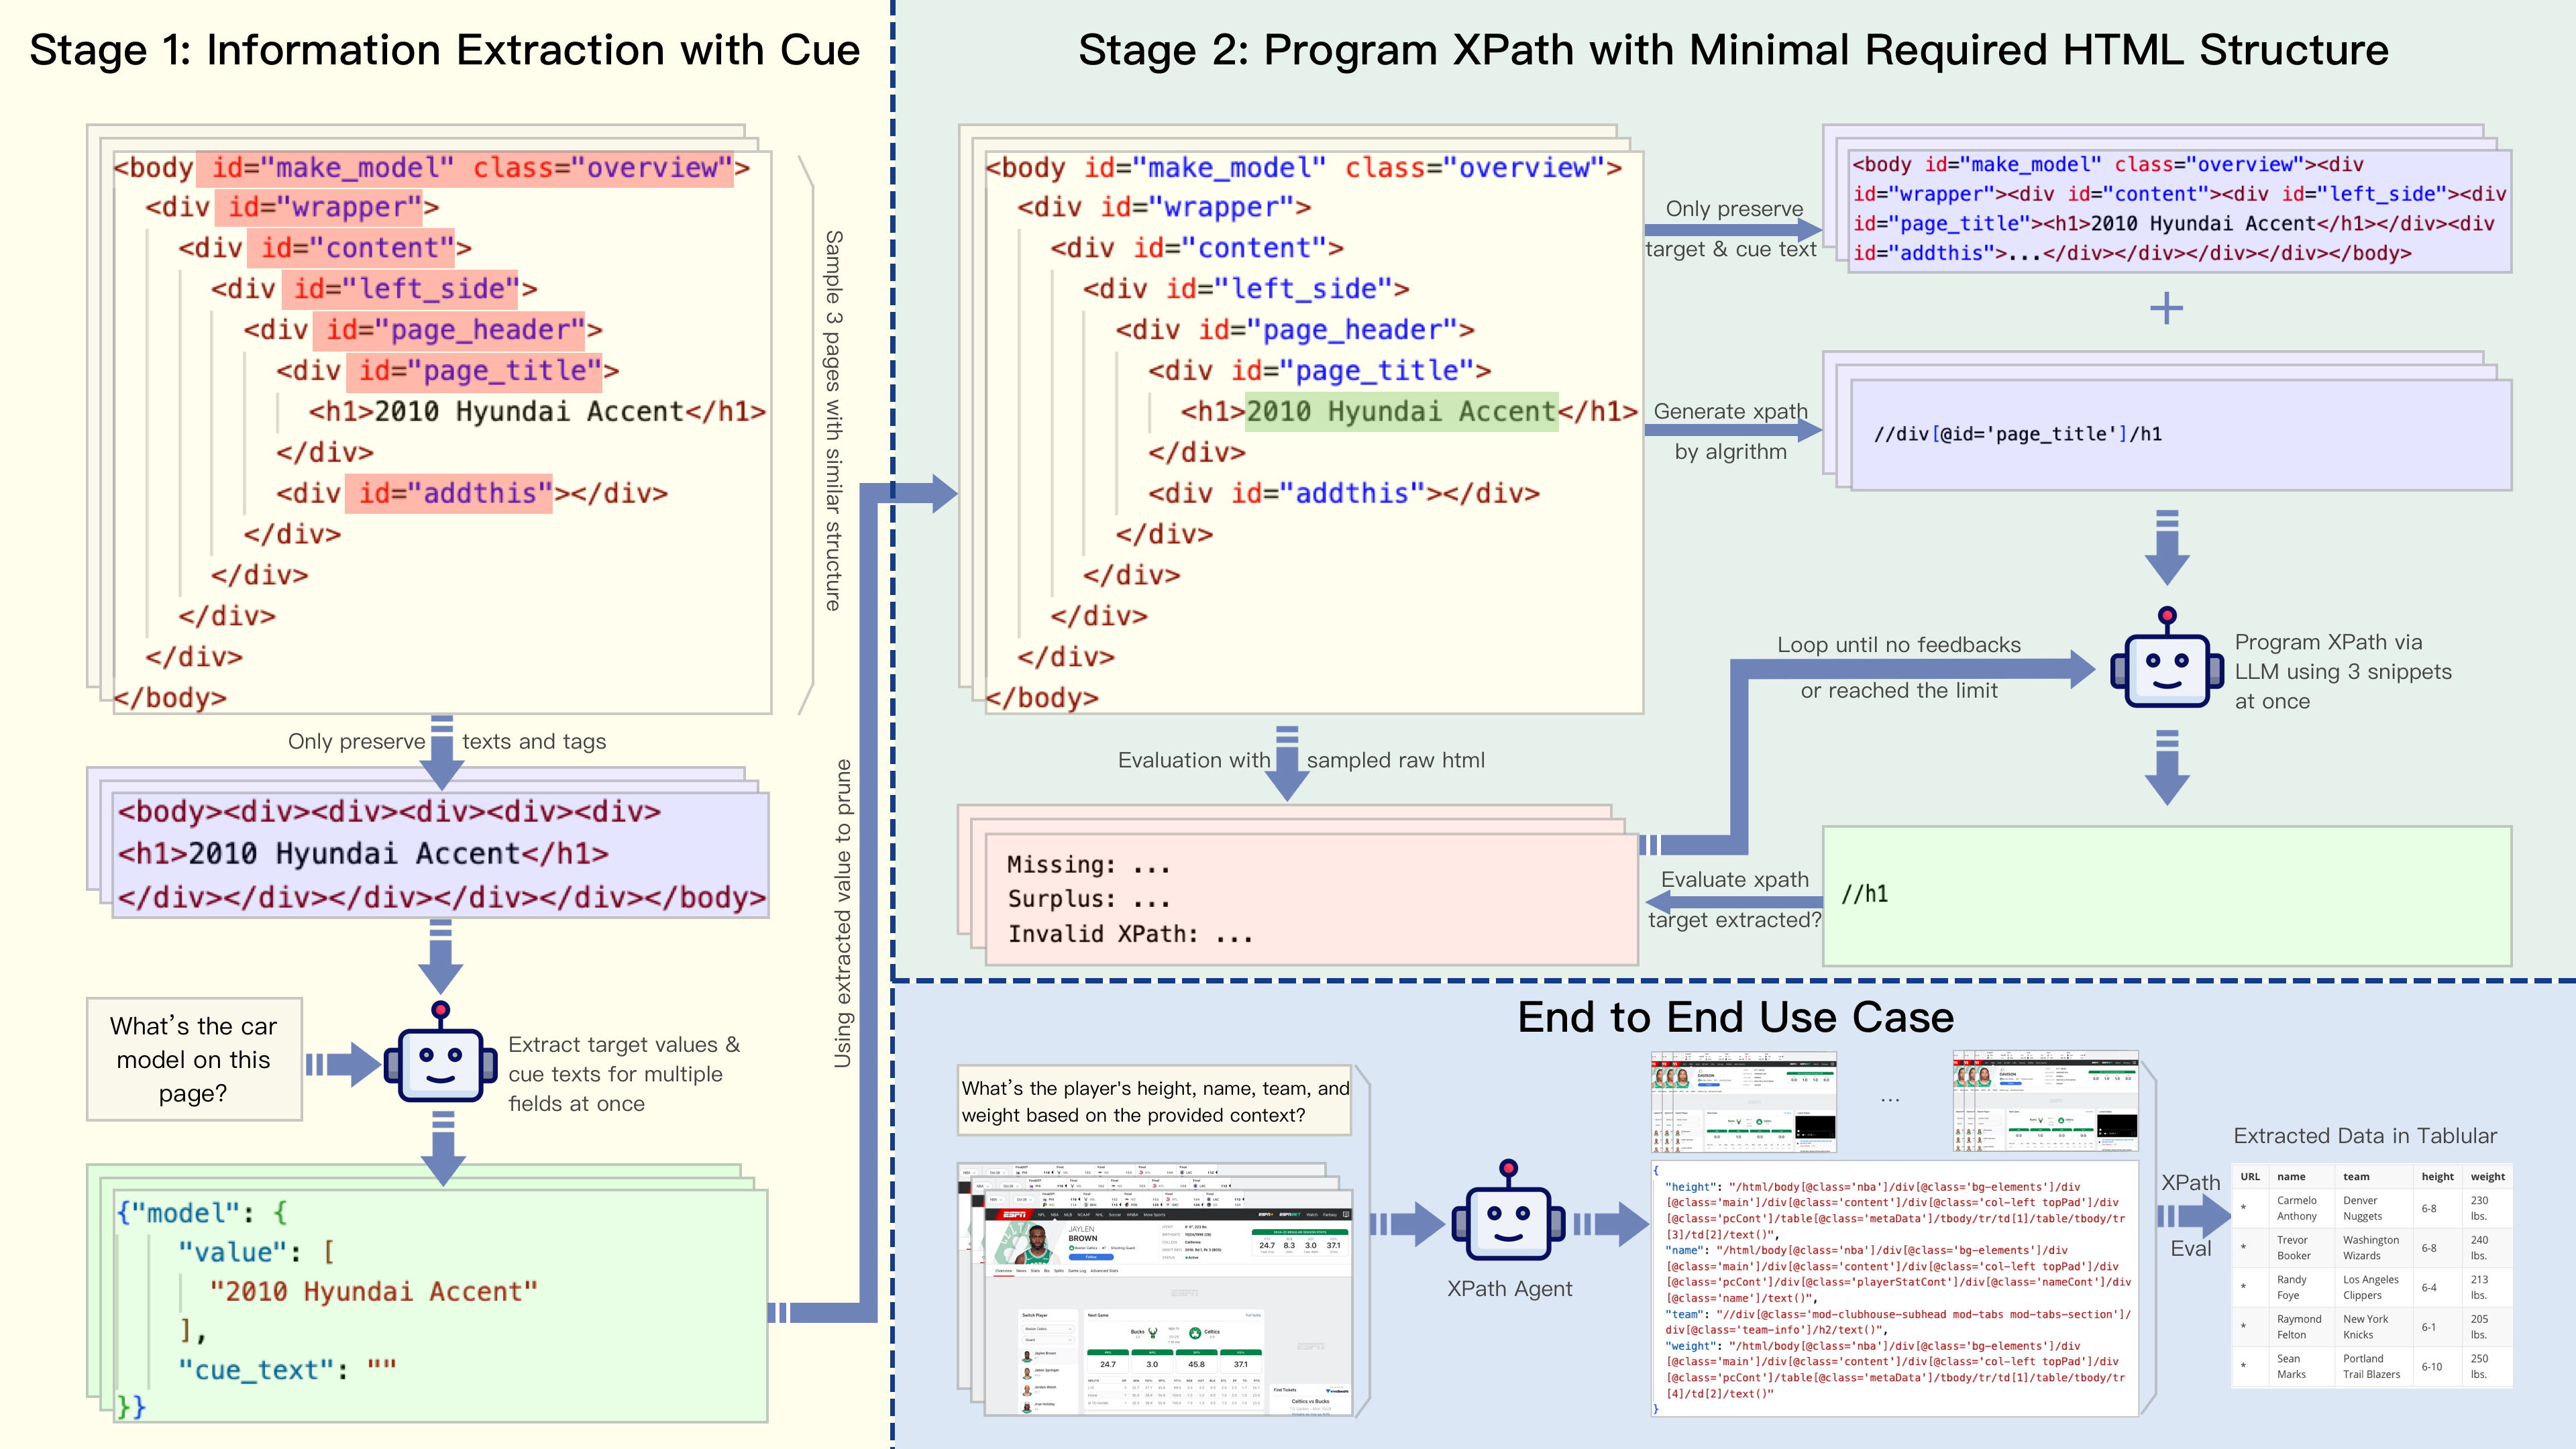
\includegraphics[width=1\textwidth]{./workflow.png}
  \caption{XPath Agent of two stages pipeline. The first stage is Information Extraction, which extracts target information and cue text from sanitized web pages (the red are sanitized). The second stage is XPath Programming, which generates XPath queries based on condensed html (the greens are target nodes) and generated XPath.}
  \label{fig:workflow}
  \vspace{20pt} % 手动插入 20pt 的垂直间距
\end{figure*}

\section{Methodology}

In this section, we present the methodology of our approach, which consists of two stages: Information Extraction (IE) and XPath Programming. The IE stage extracts target information from sanitized web pages, while the XPath Programming stage generates XPath queries based on the condensed html and extracted information. Figure \ref{fig:workflow} illustrates the two-stage pipeline of XPath Agent. For each stage, we provide a detailed description of the process and the algorithms used.

\subsection{Information Extraction with Cue Text}

The Information Extraction (IE) stage aims to extract target information. Not like traditional IE, we discovered 2 key insights. Firstly, we prompt the LLM to not only extract questioned information but also include cue texts. Secondly, we sanitized the web page to reduce the complexity of the web page and make the LLM focus on the target information.

\begin{figure}[h]
  \centering
  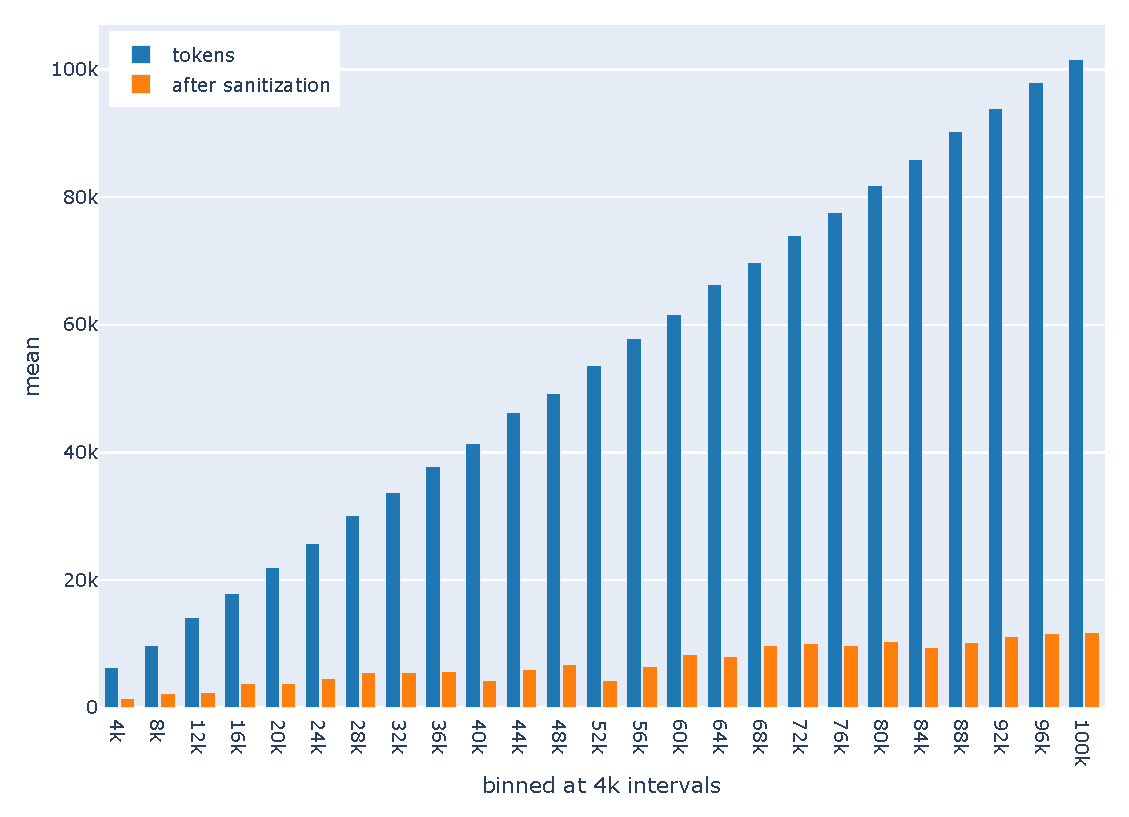
\includegraphics[width=0.5\textwidth]{./ie_token_stats.eps}
  \caption{Token Stats Analysis with Algorithm 1. As page size grow, the size after sanitization increased slowly (sampled 128 pages for each category from SWDE dataset, around 10k pages totally).}
  \label{fig:ie_token_stats}
\end{figure}

Cue texts are the indicative texts that signals the upcoming target information. For example, for "price: \$100.00", the cue text is "price:". Those texts are important in some case, especially when no way or hard to directly programming XPath queries to extract target information "\$100.00". In such case, treat "price:" as an anchor, using XPath's ancestor, sibling, or descendant axis traverse to the target information is the only way. In order to let the context still be condensed, we prompt LLM to response cue texts simultaneously.

Sanitizing web page is a process to remove unnecessary information from a page. In HTML, the most meaningful parts are texts and tags. The texts are the target information we want to extract, and the tags are the structure of the web page which tells the relationship between texts especially the priority of which answer is more likely to be the target information. The purpose of sanitizing the web page is to reduce the complexity of the web page and make the LLM focus on the target information. We designed an algorithm to sanitize the web page, which is shown in Algorithm \ref{alg:sanitizer}.

The algorithm 1 traverse the HTML tree in a depth-first manner. It removes the invisible or empty nodes, and all attributes. It's efficient and can be easily implemented in any programming language. In our sampled web pages, the algorithm can help us reduce the size of the web page to 10\%~20\% on average.

In our implementation, we prompt LLM to extract all information at once on a single page with JSON format. So, multiple fields can be extracted at the same time. Multiple values for a single field might be extracted. In this case, We simply treat all extracted values are relevant and passing them to the next stage.

\begin{algorithm}
  \SetAlgoLined
  \caption{IE HTML Sanitizer}
  \label{alg:sanitizer}
  \KwIn{Root node of HTML tree $root\_node$}
  \KwOut{Sanitized HTML tree}
  
  $left\_stack \gets [root\_node]$\;
  $right\_stack \gets []$\;
  
  \While{$left\_stack$ is not empty}{
      $node \gets left\_stack.pop()$\;
      $right\_stack.append(node)$\;
      $left\_stack \gets left\_stack + list(node.iterchildren())$\;
  }
  
  \While{$right\_stack$ is not empty}{
      $node \gets right\_stack.pop()$\;
      \If{$is\_invisiable\_or\_no\_text(node)$}{
          $node.getparent().remove(node)$\;
      }
      \Else{
          $node.remove\_attributes()$\;
      }
  }
\end{algorithm}

\subsection{XPath Program}

\begin{algorithm}
  \SetAlgoLined
  \caption{HTML Condenser}
  \KwIn{
      $root$: HTML root node\;
      $target\_texts$: List of target texts to keep\;
      $d$: Distance function between two texts\;
  }
  \KwOut{
      $root$: Condensed HTML root node\;
  }
  
  $target\_texts \gets []$\;
  $distances \gets \{\}$\;
  $eles \gets \{\}$\;
  
  \ForEach{$ele, text$ in \texttt{iter\_with\_text}($root$)}{
      \ForEach{$target\_text$ in $target\_texts$}{
          $distance \gets d(text, target\_text)$\;
          \If{$distance < distances[text]$}{
              $distances[text] \gets distance$\;
              $eles[text] \gets [\texttt{get\_xpath}($ele$)]$\;
          }
          \ElseIf{$distance == distances[text]$}{
              $eles[text].\texttt{append}(\texttt{get\_xpath}($ele$))$\;
          }
      }
  }

  $targets \gets \texttt{concat}(\texttt{values}(eles))$\;
  \ForEach{$xpath, ele$ in \texttt{iter\_with\_xpath}($root$)}{
    \If{\texttt{is\_outside}($xpath$, $targets$)}{
      \texttt{remove\_children}(ele)\;
      \texttt{replace\_text\_to}(ele, "...")\;
    }
  }

\end{algorithm}

\section{Experiments }

...

\section{Conclusion }

Third level headings must be flush left, initial caps and bold.
One line space before the third level heading and $1/2$ line
space after the third level heading.

\paragraph{Fourth Level Heading}

Fourth level headings must be flush left, initial caps and roman type.
One line space before the fourth level heading and $1/2$ line
space after the fourth level heading.

\subsection{Citations In Text}

...

\subsubsection{Footnotes}

Indicate footnotes with a number\footnote{This is a sample footnote} in
the text. Place the footnotes at the bottom of the page they appear on.
Precede the footnote with a vertical rule of 2 inches (12 picas).

\subsubsection{Figures}

All artwork must be centered, neat, clean and legible. Do not use pencil
or hand-drawn artwork. Figure number and caption always appear after the
the figure. Place one line space before the figure, one line space
before the figure caption and one line space after the figure caption.
The figure caption is initial caps and each figure is numbered
consecutively.

Make sure that the figure caption does not get separated from the
figure. Leave extra white space at the bottom of the page to avoid
splitting the figure and figure caption.

Below is another figure using LaTeX commands.



\subsubsection{Tables}

All tables must be centered, neat, clean and legible. Do not use pencil
or hand-drawn tables. Table number and title always appear before the
table.

One line space before the table title, one line space after the table
title and one line space after the table. The table title must be
initial caps and each table numbered consecutively.

\begin{table}[ht]
\begin{center}
\caption{Sample Table}

\bigskip

\begin{tabular}{|l|l|r|}
\hline
A & B & 1\\ \hline
C & D & 2\\
E & F & 3\\ \hline
\end{tabular}
\end{center}
\end{table}


\subsubsection{Handling References}

Use a first level heading for the references. References follow the
acknowledgements.


\subsubsection{Acknowledgements}

Use a third level heading for the acknowledgements. All acknowledgements
go at the end of the paper.


% \addbibresource{refs.bib}
\bibliographystyle{plain} 
\bibliography{refs}


\end{document}
